\documentclass{article}
\usepackage{graphicx} % Required for inserting images
\usepackage{amsmath}
\usepackage{amssymb}
\usepackage{amsthm}
\usepackage{todonotes}
\usepackage{stmaryrd}
\usepackage{tikz}
\usetikzlibrary{trees, positioning, arrows.meta}
%\usepackage[a4paper, total={6in, 8in}]{geometry}

\usepackage{tikz-cd} %diagramas comutativos
\usetikzlibrary{babel} %conserta compatibilidade de labels de arrows do tikz-cd
\usetikzlibrary{decorations.pathmorphing} % permite todos os tipos de arrows do tikz-cd

\newtheorem{definition}{Definition}
\newtheorem{example}{Example}
\newtheorem{theorem}{Theorem}

\newcommand{\cat}[1]{\mathsf{#1}}
\newcommand{\typesetcategory}[1]{\cat{#1}}
\newcommand{\C}{\mathcal C}
\newcommand{\Set}{\mathrm{Set}}
\newcommand{\Th}{\mathtt{Th}}
\newcommand{\QTh}{\mathtt{QTh}}
\DeclareMathOperator{\ar}{ar}

\title{Blog post 2}
\author{Anny, Augustin}
\date{April 2026}

\begin{document}

\maketitle


% This document contains the blog post (draft). 
% Roughly, we go over the definitions of the monads $\C, \C(\mathunderscore +1), \C(\mathunderscore)+1$ and $\C^\downarrow$, as well as their respective algebraic theories, giving examples of situations where one of these monads is more desirable than others for modeling purposes. Then, we present the setup of $1$-bounded metric spaces, explaining why it is useful to compute distances between programs. We also introduce the notion of lifting, and explain whether or not the previous monads can be lifted, and give examples of computation.

% \begin{table}[h]
% \centering
% \begin{tabular}{lllll}
% $\C$      & $\C(+1)$           & $\C()+1$           & $\C^\downarrow$ &  \\
% $\hat{\C}$ & $\hat{\C}(+\hat{1})$ & $\hat{\C}() +\hat{1}$ & $\hat{\C}^\downarrow$ &  \\
% \end{tabular}
% \end{table}

% Since some elements will have been introduced in the previous presentation/blog post, we can omit some details.

%\section{Blog post}

% \section{Introduction}

% In the previous post\todo{link} was introduced the idea of modeling transition systems using coalgebras $X \mapsto F(X)$, where $X$ is a set of states. Different choices of functors $F$ give us different flavors of transitions systems, and for well-behaved functors $F$, a determinization procedure induces a trace equivalence relation for the traces produced by these systems.
% These well-behaved systems are precisely the $A$-automata with $M$-effects and observations in $O$, that is, $FM$-coalgebras for the Moore-automata functor $F = O\times(\mathunderscore)^A$, where the monad $M$ determines the type of transitions.

% Consider, for example, the monad $\mathcal{C}$ of non-empty finitely generated convex sets of probability distributions. Intuitively, $\mathcal{C}$ models nondeterministic choice followed by probabilistic choice. (Note that $\mathcal{C}$ is not simply the composition of the classical monads for nondeterminism and probability choice, since there is no distributive law to compose them.)

%     Rather than describing explicitly the unit and the multiplication of $\C$, we can use a presentation of $\C$: an algebraic theory $(\Sigma, E)$, where $\Sigma$ is a signature (a set of symbols with prescribed arity) and $E$ is a set of equations (the axioms of the theory), such that $\C$ is isomorphic to the term monad $T_{(\Sigma, E)}$, the $\Set$-monad mapping a set of variables $X$ to the set of $\Sigma$-terms with variables in $X$, modulo equations in $E$. 

%     Equivalently, this says that there is a concrete equivalence between the Eilenberg-Moore category of $\C$-algebras and the category of models of the theory $(\Sigma, E)$, whose objects are sets $A$ equipped with an interpretation $\llbracket\sigma\rrbracket: A^{\ar(\sigma)} \to A$ that respects the axioms of the theory.

%     Handling $\C$ via a presentation is very convenient, since it provides an equational tool to understand and reason about $\C$. For instance, to determinize an automata with $\C$-effects and observations in $O$, the set $O$ must be a $\C$-algebra. A presentation of $\C$ tells use exactly what structure $O$ must carry. 
%     Fortunately, it was proved in \cite{Bonchi_2022} that the following theory presents $\C$:

% \begin{definition}
% $\Th_{CS}$ is the theory of convex semilattices, with signature $\Sigma_{CS} = (\{\oplus\} \cup \{+_p\}_{p \in (0,1)})$, and the axioms:
%     \begin{align*}
% &\text{(A)} && x \oplus (y \oplus z) = (x \oplus y) \oplus z \\
% &\text{(C)} && x \oplus y = y \oplus x \\
% &\text{(I)} && x \oplus x = x \\
% &\text{(A}_p\text{)} && (x +_q y) +_p z = x +_{pq} (y +_{\frac{1-q}{1-p}} z) \\
% &\text{(C}_p\text{)} && x +_p y = y +_{1-p} x \\
% &\text{(I}_p\text{)} && x +_p x = x \\
% &\text{(D)} && x +_p (y \oplus z) = (x +_p y) \oplus (x +_p z)
% \end{align*}
% \end{definition}
% Intuitively, $\oplus$ represents nondeterministic choice while $+_p$, $p\in(0,1)$ represents probabilistic choice.
% Using this presentation, we can for example handle the faulty vending machine:

% \begin{center}
%     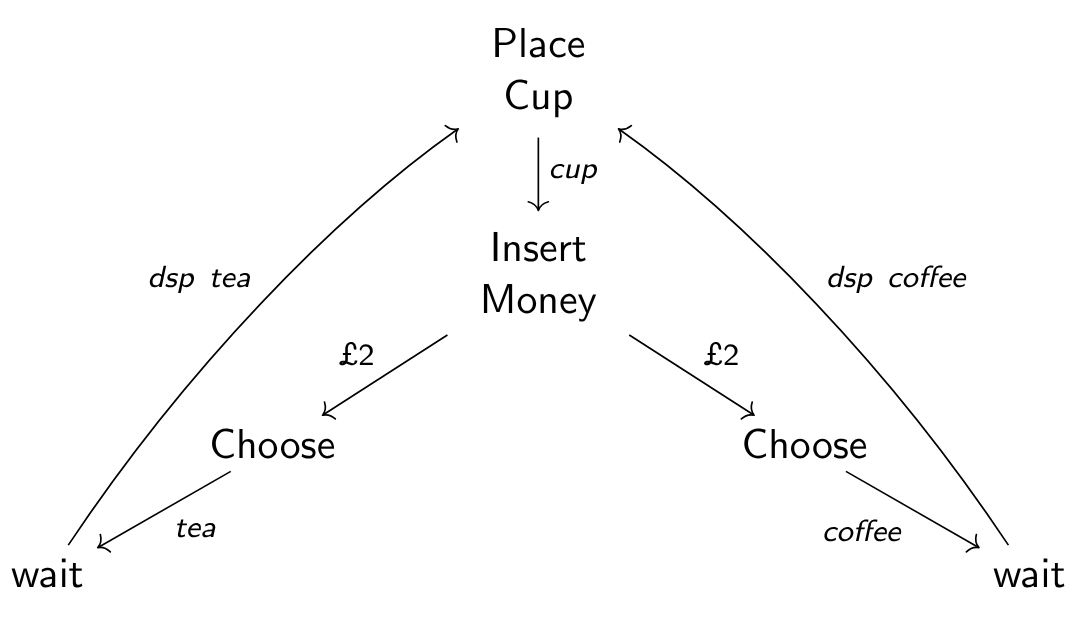
\includegraphics[width=8cm]{faulty.png}
% \end{center}
% To fit into the framework of automatas, we consider a trivial set of observation $O = \{*\}$, the alphabet $A = \{\textsf{cup}, \ldots\}$ and the monad $C$. A final state $\bullet$, not depicted on the figure, is the target of the transitions that are not depicted. Using the presentation of $\C$, we can describe the following trace in the determinization of the automata using the finite syntax:
% $$  \textsf{Place Cup} \xrightarrow{\textsf{cup}} \textsf{Insert Money} \xrightarrow{\textsf{\pounds 2}} \textsf{Choose} \oplus \textsf{Choose} \xrightarrow{\textsf{tea}} \textsf{wait} \oplus \bullet$$

% \section{Modeling termination}

% The monad $\C$ alone does not account for termination. Instead, we can combine $\C$ with the termination monad $+1$, which maps a set $X$ to $X\sqcup{\star}$, where the extra element $\star$ represents termination. There are two distributive laws between $\C$ and $+1$: 
% \begin{align*}
%     \C+1 \Rightarrow \C( +1)\\
%     \C( +1) \Rightarrow \C+1
% \end{align*}
% The first law exists for any monad $M$:

% \begin{definition}
% Let a category $\cat{C}$ have coproducts and a terminal object $1$, and let $(M, \eta, \mu)$ be a $\cat{C}$-monad. There is a distributive law $\iota \colon M+1 \Rightarrow M(+1)$ defined as :
% \[
% \iota_X = [M \operatorname{inl}, \; \eta_{X+1} \circ \operatorname{inr}]
% \]
% where $\operatorname{inl} : X \to X+1$ and $\operatorname{inr} : 1 \to X+1$ are the coproduct injections for $X+1$. 
% \end{definition}

% Intuitively, $\iota$ interprets "either run a $M$-computation with effects in $M$ or terminate" as "run a computation with effects in $M$ that can terminates". This yields the monad $\C(+1)$ of of non-empty finitely generated convex sets of
% subdistributions, which admits as presentation the theory $\Th_{C S}^*$, which is $\Th_{C S}$ with an added symbol $*$ of arity $0$, and the same equations.

% The second distributive law is more specific to $\C$:

% \begin{definition}
%     For every set \( X \), the map \( \gamma_X : C(X + 1) \to C(X) + 1 \) is defined as follows, for any \( S \in C(X + 1) \):
% \[
% \gamma_X(S) =
% \begin{cases} 
% \{\varphi \mid \varphi \in S \text{ and } \varphi(\star) = 0\} & \exists \varphi \in S \text{ s.t. } \varphi(\star) = 0 \\
% \star & \text{otherwise}
% \end{cases}
% \]
% \end{definition}

% Intuitively, $\gamma_X(S)$ maps a non-empty finitely generated convex set of probability subdistributions to its convex subset of full distributions if its not empty, or to $\star$ otherwise. This gives the monad $\mathcal{C} +1$, whose underlying functor is the well-known convex Segala systems functor.

% The two monads model termination differently:

% \begin{itemize}
%     \item In $\C(+1)$, probabilistic choice can lead to termination (a subdistribution can have mass less than 1).
%     \item In $\C+1$, termination is a global, nondeterministic alternative: a state either transitions to a proper CC-computation or terminates outright.
% \end{itemize}

% One of the main results of the paper is a presentation for $\mathcal{C}+1$. 

% \begin{theorem}\label{th:pres_bot_bh}
% The monad $\C(+1)$ is presented by the theory $\Th_{C S}^{\bot, BH}$, which extends $\Th_{C S}^*$ with the axioms \( \bot = \{x \oplus \star = x\} \)  
% and \( BH = \{x +_p \star = \star \mid p \in (0, 1)\} \).
% \end{theorem}
% The bottom axiom $(\bot)$ says that nondeterministically choosing between a continuation $x$ and termination is equivalent to $x$ alone. The black-hole axiom ($BH$) says that probabilistically choosing between $x$ and termination with any non-zero probability results in termination.

% This last axiom may be too strong for certain modeling purposes.
% Could we consider instead the theory  $\Th_{C S}^{\bot}$ which only keep the bottom axiom ? The paper answer this by showing that $\Th_{C S}^{\bot}$ presents the monad $\C^\downarrow$ of non-empty finitely generated $\bot$-closed convex sets of probability subdistributions. A set $S$ of subdistributions is $\bot$-closed if whenever $\phi\in S$, any subdistribution $\psi$ with $\psi(x) \leq \phi(x)$ for all $x$ (more chance of termination) also belongs to $S$. 

% Now that we know how to model termination in different ways, lets see these monads in action on a minimalist programming language. Let us consider the following process algebra $Proc$. Process terms are defined by:
% $$ P ::= \mathbf{nil} \ | \  P_1 \overline \oplus P_2\ |\  P_1 \overline +_p P_2\ | \ a.P, a \in A$$
% where $A$ is a set of labels.

% Here, $\mathbf{nil}$ is the terminated process and $a.P$ performs action $a$ and continue as $P$. Intuitively, a program can execute some actions in $A$ or branch in a nondeterministically or probabilistic manner. However, it remains to define precisely the transition semantics of these processes (essentially the semantics for branching).

% We now define inductively an operational semantics on process terms, by assigning to each term $P$ its continuation $t \in T_{\Th^{*}_{CS}}(Proc) \cong \C(Proc+1)$, denoted $P \rightarrowtail t$: a term in the free model of $\Th^{*}_{CS}$ over process terms, representing the control flow of the program.

% \begin{align*}
% &\frac{}{a.P \rightarrowtail P}
% &\frac{}{\mathbf{nil} \rightarrowtail \star} \ & 
% &\frac{P_1 \rightarrowtail t_1 \ \ P_2 \rightarrowtail t_2}{P_1 \oplus P_2 \rightarrowtail t_1 \oplus t_2}\ &
% &\frac{P_1 \rightarrowtail t_1 \ \ P_2 \rightarrowtail t_2}{P_1 +_p P_2 \rightarrowtail t_1 +_p t_2}
% \end{align*}

% Without further modifications, this operational semantics yields the transition semantics (coalgebras) $Proc \to \C(Proc+1)$. However, we can also quotient the continuation of process terms by additional equations to obtain rougher equivalence classes of programs.

% Now, depending on which equational theory we quotient the continuations by, we obtain different transition semantics (coalgebras) $Proc \to F(Proc)$:
% \begin{itemize}
%     \item Quotienting by $(\bot)$ gives the transition semantics $Proc \to \C^\downarrow(Proc)$.
%     \item Quotienting by $(\bot)$ and $(BH)$ gives the transition semantics $Proc \to \C(Proc)+1$.
% \end{itemize}

% Consider for example the program
% $P = a.(b.\mathbf{nil} +_{\frac12} \mathbf{nil}) \oplus \mathbf{nil}$.

% The three transition semantics of $P$ are depicted below. Intuitively, without the bottom axiom, the program can terminate without executing $b$. The black hole axiom, on the other hand, prevent from executing  $b$ altogether.

% 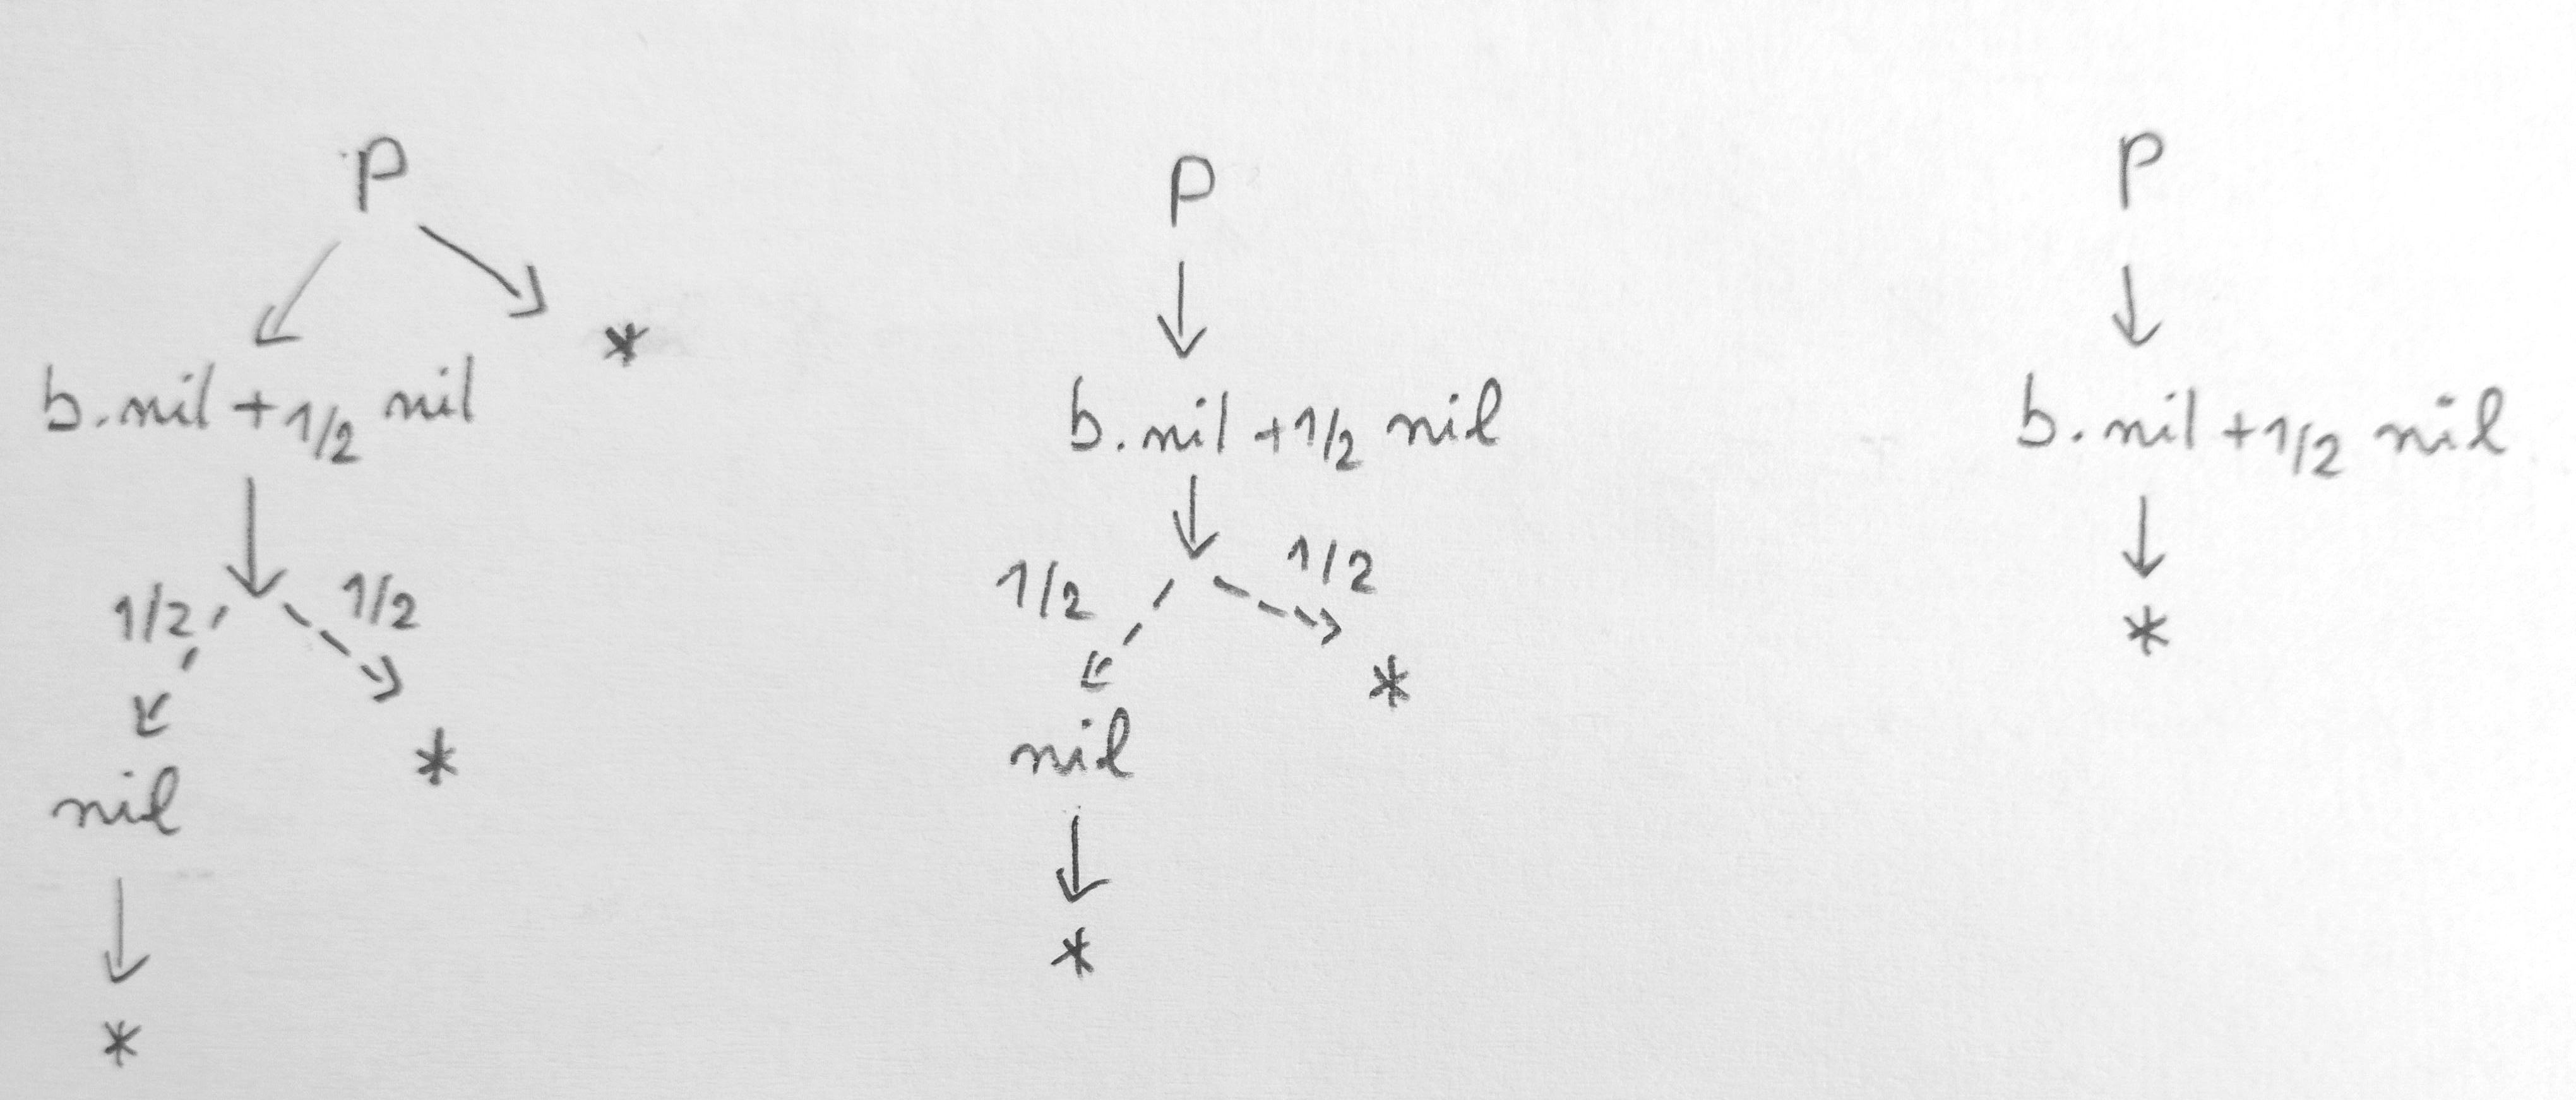
\includegraphics[width=10cm]{traces.png}

% The choice of transition semantics thus necessarily impact equivalences between programs. Another benefit of monads presentations, is to show that two programs $P_1$ and $P_2$ are behaviorally equivalent under some transition semantics, it suffice to show that their continuation are equal in the relevant presentation.

% For example, $P$ and $a.(b.\mathbf{nil} +_{\frac12} \mathbf{nil})$ are provably equal, i.e. behaviorally equivalent, for the transition semantics  $Proc \to \C^\downarrow(Proc)$ and  $Proc \to \C(Proc)+1$, but not for $Proc \to \C(Proc+1)$!

Remember the Pacman game from the blog post~\todo{TODO cite previous blog post}? The authors applied a determinization procedure to it, but did not draw the resulting coalgebra. In this post, we introduce different algebraic presentations of monads that model nondeterminism and probability in order (among other niceties) to draw that determinized automaton. Determinization is the first step for computing equivalences of automata. In the second part of this blog, we go beyond equalities and define a distance between automata, without losing our previously defined
$\cat{Set}$-monads, nor their presentations.

\section{Algebraic presentations of monads for automata }

This blog post builds on the great post~\todo{link to the blog by Alyssa and Max}, and we advise reading it before proceeding. In that post, we learned how transition systems can be modeled as coalgebras $S \to F(S)$, with $S$ a set of states and $F$ a functor. We also encountered automata and a notion of equivalence between automata given by determinization followed by bisimulation. Recall that an automaton with $M$-effects, labels in $A$, and observations in $O$ is a coalgebra $S \to O \times (MS)^A$. Each transition is given a label from the set $A$, the set $O$ describes all the observations one can make about a state in $S$, and the functor $M$ gives some flavor to the transitions...

%determinization \(O\) 



Consider for example the monad \(\mathcal{C}\) of non-empty finitely generated convex sets of probability distributions. Intuitively, \(\mathcal{C}\) models nondeterministic choice followed by probabilistic choice. For example, we can model Alyssa's Pacman game! %(Note that \(\mathcal{C}\) is not simply the composition of the classical monads for nondeterminism and probability, because there is no distributive law to compose them!)

\begin{center}
    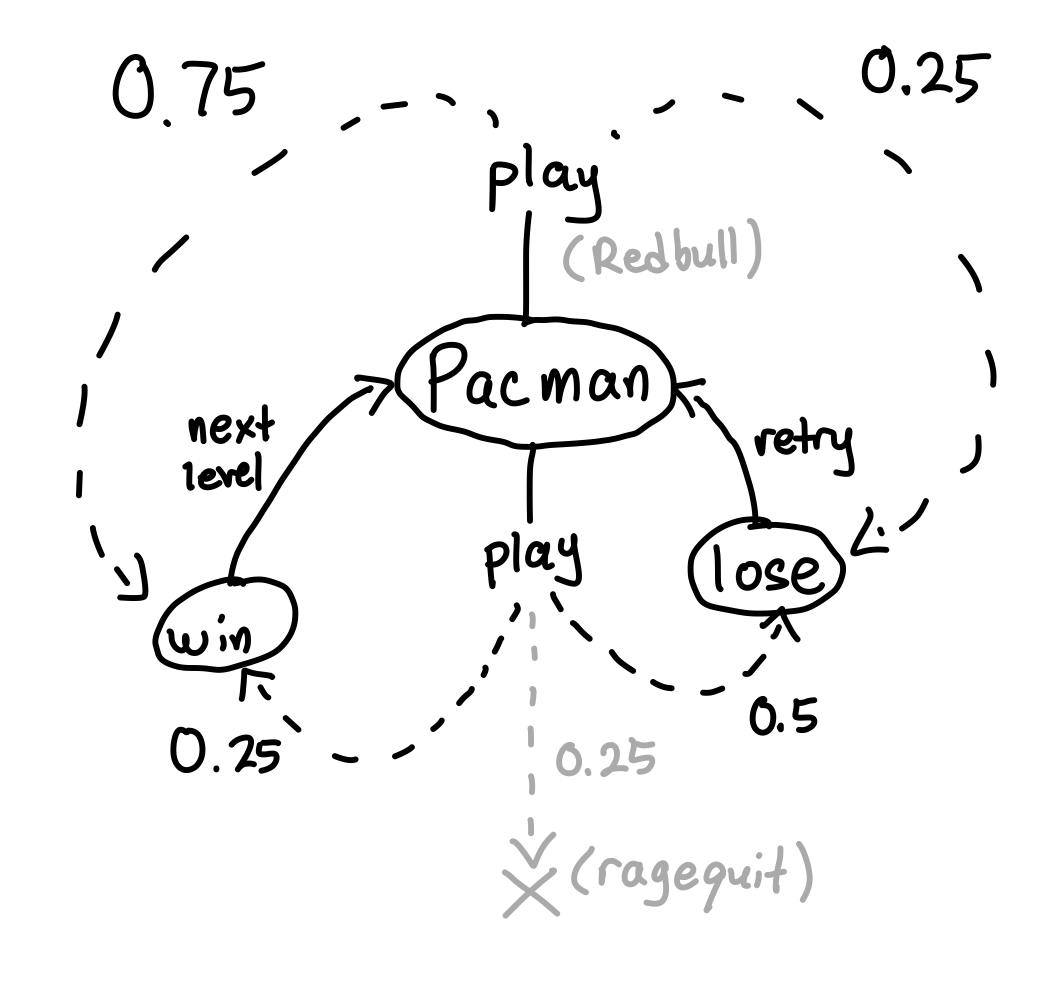
\includegraphics[width=.4\textwidth]{pacman.png}
\end{center}


Rather than writing down unit and multiplication explicitly, we will use a \emph{presentation} of \(\mathcal{C}\): an algebraic theory \((\Sigma, E)\) such that \(\mathcal{C}\) is isomorphic to the monad mapping sets of variables to \(\Sigma\)-terms modulo \(E\). Intuitively, a presentation of $M$ is to algebras of $M$ what the theory of rings is to rings. The $M$-algebras are \emph{models} of  the presentation.

%Equivalently, the Eilenberg-Moore category of \(\mathcal{C}\)-algebras is concretely equivalent to the category of models of \((\Sigma, E)\) (e.g. models of the theory of rings are simply rings!).

We will see that handling \(\mathcal{C}\) via a presentation is very convenient. %as it gives equational tools to reason about \(\mathcal{C}\). 
For instance, to determinize an automaton with \(M\)-effects and \(O\)-observations, we need an algebra \(MO \to O\). A presentation tells us exactly what structure \(O\) must carry! 

For $\C$, it was shown in~\todo{cite paper(s)!} that this monad is presented by the theory of convex semilattices, whose signature
is made of a binary operation \(\oplus\) (nondeterministic choice), and for each \(p \in (0,1)\) a binary operation \(+_p\) (probabilistic choice with probability \(p\)), and whose axioms are:
\[
\begin{aligned}
&\text{(A)} && x \oplus (y \oplus z) = (x \oplus y) \oplus z \\
&\text{(C)} && x \oplus y = y \oplus x \\
&\text{(I)} && x \oplus x = x \\
&\text{(A}_{q,p}\text{)} && (x +_q y) +_p z = x +_{pq} (y +_{\frac{1-q}{1-p}} z) \\
&\text{(C}_p\text{)} && x +_p y = y +_{1-p} x \\
&\text{(I}_p\text{)} && x +_p x = x \\
&\text{(D)} && x +_p (y \oplus z) = (x +_p y) \oplus (x +_p z)
\end{aligned}
\]

With a presentation of $\mathcal C$, we get a language to describe the new states of the determinization of a $\mathcal C$-automaton: each determinized state is a finite expression made of the original states and the operations in the signature like  $\mathtt{Pacman}$ or $\mathtt{win} +_{3/4} \mathtt{lose}$. The presentation tells us how to compute the transitions:
For ``simple'' states like $\mathtt{Pacman}$, we just read from the automaton the expression corresponding to the right combination of nondeterminism and probability:
 \begin{align*}
     &\mathtt{Pacman}\\
    &\downarrow \mathtt{play}\\
    (\mathtt{win} +_{0.75} \mathtt{lose}) \oplus  &((\mathtt{win} +_{0.5} \star) +_{0.5} \mathtt{lose})\\ 
\end{align*}

For ``complex'' states like the one above, the theory of presentations tell us that  %\todo{ana: may be misleading} 
every occurrence of simple states can be replaced by the complex state it transitions to, e.g.:

\begin{align*}
    (\mathtt{win} +_{0.75} \mathtt{lose}) \oplus  &((\mathtt{win} +_{0.5} \star) +_{0.5} \mathtt{lose})\\
    & \downarrow \mathtt{next\ level}\\
    (\mathtt{Pacman} +_{0.75} \star) \oplus  &((\mathtt{Pacman} +_{0.5} \star) +_{0.5} \star)
\end{align*}

Finally, we can use the equations of the presentation to simplify this expression a bit:

\begin{align*}
    (&\mathtt{Pacman} +_{0.75} \star) \oplus  ((\mathtt{Pacman} +_{0.5} \star) +_{0.5} \star)\\
    &= (\mathtt{Pacman} +_{0.75} \star) \oplus  (\mathtt{Pacman} +_{0.25} (\star +_{1} \star) & ({A}_{0.5, 0.5})\\
    &= (\mathtt{Pacman} +_{0.75} \star) \oplus (\mathtt{Pacman} +_{0.25} \star) & (\text{I})
\end{align*} 

% We call this theory \(\Th_{CS}\).
% With this presentation of $\mathcal C$, we can for example describe the faulty vending machine pictured below. 

% \begin{center}
%     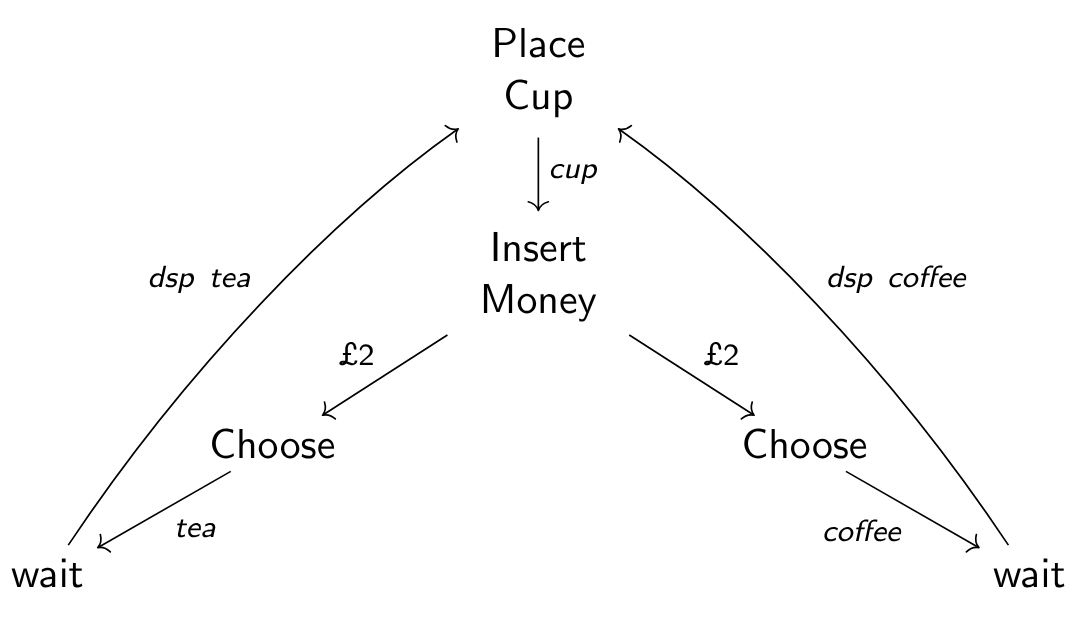
\includegraphics[width=8cm]{faulty.png}
% \end{center}

% Consider a trivial set of observation \(O = \{*\}\), the alphabet \(A = \{\textsf{cup}, \ldots\}\) and the monad \(\mathcal{C}\). The automaton also has an hidden sink state $\star$. We can now denote the states of the determinized automaton using the algebraic theory \(\Th_{CS}\), consider for example the following trace:
% \[
% \textsf{Place Cup} \xrightarrow{\textsf{cup}} \textsf{Insert Money} \xrightarrow{\textsf{\pounds 2}} \textsf{Choose} \oplus \textsf{Choose} \xrightarrow{\textsf{tea}} \textsf{wait} \oplus \star
% \]


\subsection{Modeling termination.}
The way we modeled ragequit and actions not applying on certain states using a terminal state $\star$ is a bit ad hoc, though. A more systematic way of modeling termination (e.g., a program returning or crashing) which also behaves better with more complex sets of observations, is to compose the monad $M$ modeling certain effects with the $+1$ termination monad, which acts on sets by adding a distinct element $\star$ representing termination. This yields a new monad $M(+1)$. Having a monad is useful: we can use the same automaton formalism, but with termination. 
%to   \(+1: X \mapsto X \sqcup \{\star\}\), where \(\star\) \todo{ana:$\sqcup$ is bad here, +}signals termination. 
%Indeed, there is always a monad distributive law \(\iota \colon M+1 \Rightarrow M(+1)\). 
For $\mathcal C$, this gives the monad \(\mathcal{C}(+1)\) of non-empty finitely generated convex sets of \emph{subdistributions}, i.e., a probability distribution whose total mass is less or equal to $1$ (instead of exactly $1$).

Interestingly, this monad is presented by the theory of \emph{pointed} convex semilattices, i.e., we add an extra symbol $\star$ in the signature with no additional equations. 

However, there are different ways to model termination with the monad $\mathcal C$: for example, termination may be a nondeterministic alternative: a state either transitions to a non-terminating effectful state, or terminates outright. In our example, however, termination is probabilistic: some actions have a chance to lead to termination every time they are applied.


This is another point where algebraic presentations shine: it is easy to add additional axioms to the theory of pointed convex semilattices to refine the meaning of termination, and it again gives a presentation of some monad. However, there is not always a nice semantic description of these monads... Nevertheless, it does when adding either the bottom axiom $(\bot)$, or both $(\bot)$ and the black hole axiom $(BH)$!
\begin{align*}
    &\{x \oplus \star = x\}\ (\bot) &\{x +_p \star = \star \mid p \in (0, 1)\}\ (BH)
\end{align*} %\todo{ana:unusual way of writing axioms, better is axiom and then ($\bot$) - not in a set}
The resulting monads are called $\mathcal C+1$ and $\mathcal C^\downarrow$.
    
% For the two following well known axioms $(\bot)$ and $(BH)$, we again  

% % The monad \(\mathcal{C}\) alone does not account for termination. We got away with a terminal state $\star$ in the Pacman game, but it was because we did not care about observations! If we had chosen a non trivial set of observations, things would have gone wrong... Consider for example observations in $[0,1]$ measuring the happiness of a player at each state. We explicitly assign $0$ to the terminal state $\star$. $\mathcal C$


% % but we can combine it with the termination monad \(+1: X \mapsto X \sqcup \{\star\}\), where \(\star\) signals termination. There are two distributive laws between \(\mathcal{C}\) and \(+1\), giving two different combined monads.

% % The first distributive law exists for any monad \(M\): \(\iota \colon M+1 \Rightarrow M(+1)\), interpreting ``either run an \(M\)-computation or terminate'' as ``run an \(M\)-computation that may terminate''. This yields the monad \(\mathcal{C}(+1)\) of non-empty finitely generated convex sets of \emph{subdistributions}. Its presentation is the theory \(\Th_{CS}^*\), obtained by adding a constant symbol \(*\) (representing \(\star\)) to \(\Th_{CS}\) with no extra equations.

% The second distributive law is specific to \(\mathcal{C}\). For any set \(X\), define \(\gamma_X \colon \mathcal{C}(X+1) \to \mathcal{C}(X)+1\) by sending a convex set \(S \in \mathcal{C}(X+1)\) to its subset of full distributions (those assigning probability \(0\) to \(\star\)) if that subset is nonempty, and to \(\star\) otherwise. This gives the monad \(\mathcal{C}+1\), whose underlying functor is the convex Segala system functor.

% The two monads model termination differently: in \(\mathcal{C}(+1)\), probabilistic choice can lead to termination (a subdistribution may have total mass \(<1\)), whereas in \(\mathcal{C}+1\), termination is a global, nondeterministic alternative: a state either transitions to a proper \(\mathcal{C}\)-computation or terminates outright.

% One of the main results of the paper is a presentation for \(\mathcal{C}+1\): the theory \(\Th_{CS}^{\bot, BH}\) extends \(\Th_{CS}^*\) with the bottom axiom \(\bot = \{x \oplus \star = x\}\) and the black-hole axiom \(BH = \{x +_p \star = \star \mid p \in (0, 1)\}\). The bottom axiom means that nondeterministically choosing between \(x\) and termination is just \(x\). The black-hole axiom says that probabilistically choosing between \(x\) and termination with any positive probability results in termination.

% This black-hole axiom may be too coarse for some systems. Could we then keep only the bottom axiom? It turns out that \(\Th_{CS}^{\bot}\) presents the monad \(\mathcal{C}^\downarrow\) of non-empty finitely generated \(\bot\)-closed convex sets of subdistributions, where a set \(S\) is \(\bot\)-closed if whenever \(\phi \in S\), any subdistribution \(\psi\) with \(\psi(x) \le \phi(x)\) for all \(x\) also belongs to \(S\).

% \paragraph{Process algebras}
% To see these monads in action, consider the following minimal process algebra \(Proc\):
% \[
% P ::= \mathbf{nil} \mid P_1 \mathbin{\overline{\oplus}} P_2 \mid P_1 \mathbin{\overline{+}_p} P_2 \mid a.P, \quad a \in A
% \]
% Here, \(\mathbf{nil}\) represents the terminated process, \(a.P\) performs action \(a\) and continues as \(P\), and  \(\overline{\oplus}\) and \(\overline{+}_p\) are nondeterministic and probabilistic branchings, respectively.

% We give a more formal semantics to these processes, we inductively assign to each process \(P\) a continuation \(t \in T_{\Th_{CS}^*}(Proc) \cong \mathcal{C}(Proc+1)\), written \(P \rightarrowtail t\):
% \[
% \frac{}{a.P \rightarrowtail P} \qquad
% \frac{}{\mathbf{nil} \rightarrowtail \star} \qquad
% \frac{P_1 \rightarrowtail t_1 \quad P_2 \rightarrowtail t_2}{P_1 \mathbin{\overline{\oplus}} P_2 \rightarrowtail t_1 \oplus t_2} \qquad
% \frac{P_1 \rightarrowtail t_1 \quad P_2 \rightarrowtail t_2}{P_1 \mathbin{\overline{+}_p} P_2 \rightarrowtail t_1 +_p t_2}
% \]
% Intuitively, the continuation of a process is a syntactic object representing the control flow of the program once it has executed an instruction.
% This yields our semantics, a transition coalgebra \(Proc \to \mathcal{C}(Proc+1)\). By quotienting the continuation terms with additional equations, we obtain different transition semantics:
% \begin{itemize}
%     \item quotienting by \((\bot)\) gives \(Proc \to \mathcal{C}^\downarrow(Proc)\),
%     \item quotienting by both \((\bot)\) and \((BH)\) gives \(Proc \to \mathcal{C}(Proc)+1\).
% \end{itemize}

% Consider now the program
% \(P = a.(b.\mathbf{nil} +_{\frac12} \mathbf{nil}) \mathbin{\overline{\oplus}} \mathbf{nil}\).
% Without the bottom axiom, \(P\) can terminate without ever executing \(b\), and with the black-hole axiom, the possibility of executing \(b\) is killed entirely. Graphically, the three transition semantics for \(P\) are:

% 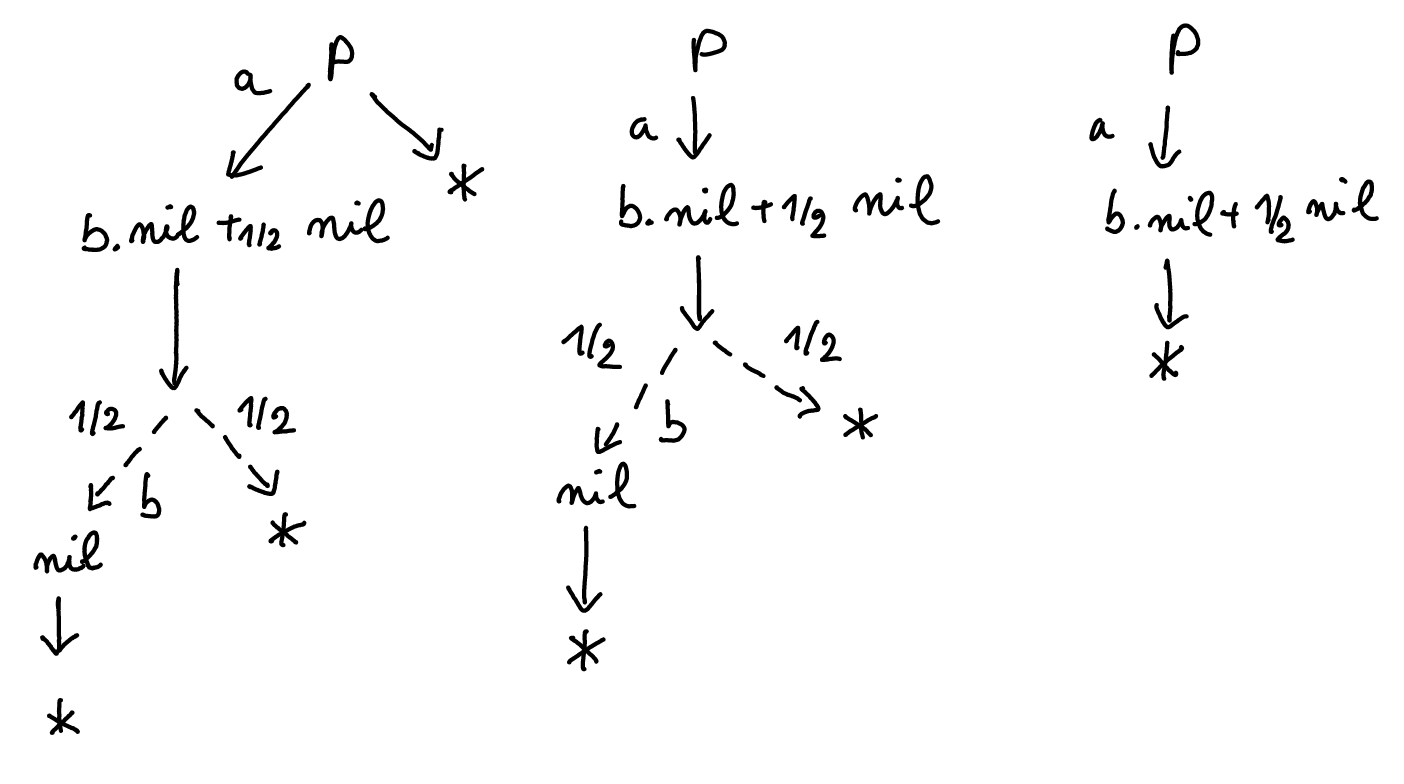
\includegraphics[width=10cm]{traces2.png}

% Each choice of transition semantics induces a notion of equivalence of processes. A major benefit of monad presentations is that to prove two processes \(P_1\) and \(P_2\) are behaviorally equivalent under a given semantics, it suffices to show that their (iterated) continuations are equal in the relevant equational theory. For instance, the continuations \(P\) and \(a.(b.\mathbf{nil} +_{\frac12} \mathbf{nil})\) are provably equal, hence behaviorally equivalent, in the semantics \(Proc \to \mathcal{C}^\downarrow(Proc)\) and \(Proc \to \mathcal{C}(Proc)+1\), but \emph{not} in \(Proc \to \mathcal{C}(Proc+1)\).

\section{From equivalences to distances between automata}%\todo{ana:singular: automaton, plural: automata. Yes, I think t should be plural in the section title, unless i(m mistaken?}

%\subsection{Example (why should we care about program distance)}
Now here comes the best part: while equivalences of automata are nice, distance between programs are even nicer, and sometimes necessary to reason properly about programs with probability and nondeterminism! Our intuition tells us that programs that return the same output with high-probability should be closer than programs whose output are different almost all the times. Distances make this intuition formal by using quantities (usually real numbers) to represent how close/far programs are.
% Why consider metric spaces and distances between programs? Equivalence is often too coarse. In some cases we may want to know how different two programs are, e.g., the probability that they produce different outputs, or the `cost' of one optimization over another. Distances provide this quantitative measure.

Consider for example the following transition system (from \cite[Section 2]{coalg-metrics}), without labels, and with state space $X = \{u,x,y,z\}$, where $\varepsilon \in [0,0.5]$, $z$ is an accepting state and $u$ is a fail state, which once reached can never be left and the system loops indefinitely.

\begin{figure}[h]
    \centering
    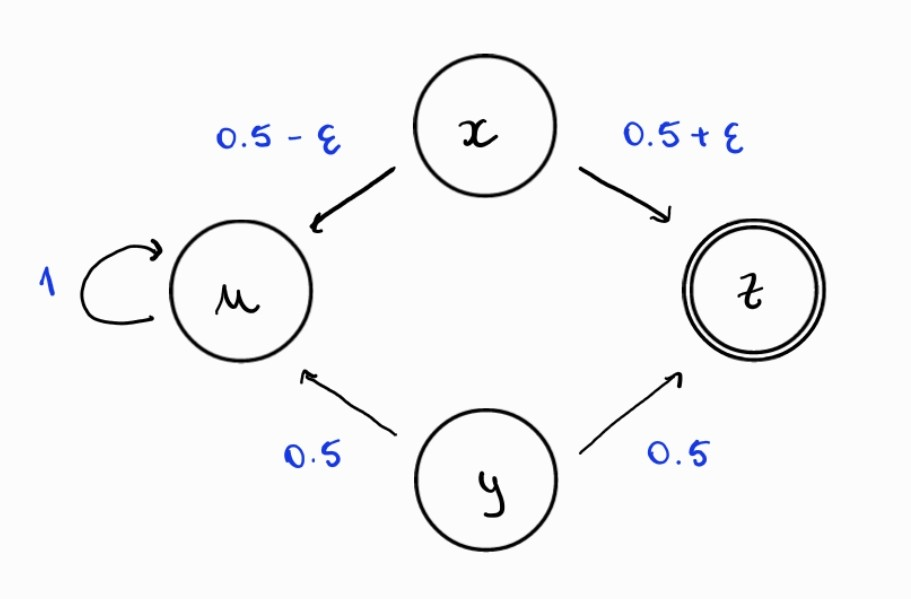
\includegraphics[width=0.5\linewidth]{images/pts.jpg}
    % \caption{Transition system with four states}
    % \label{fig:1}
\end{figure}
%I think that you should not bother with figures, since they are going to be scrapped with the switch to markdown for the blog post! Just put the image maybe!

If we compare the behavior of $x$ and $y$, we see that they are not behaviorally equivalent. This is because in state $x$ there is always a bias towards the accepting state $z$ which is controlled by the value of $\varepsilon$. However, we would like to say that their behavioral distance is$\varepsilon$. % But, they are similar in the sense that their \todo{ana:this sounds as if there is "the" beh.distance. AA:changed the formulation a bit...} behavioral distance is $\varepsilon$. 
If we took $\varepsilon = 0$, then they would really be behaviorally equivalent.
In the rest of this post, we will show how to formalize this notion of distance without losing the benefits of presentations!
To begin with, we will need to work with monads in $\cat{1Met}$ rather than $\cat{Set}$ in order to get a notion of distance.

%saw that we could use the $\cat{Set}$-monad $\C$ to reason about systems that combine nondeterminism and probability. In order to capture the notion of distances, we will use monads in $\cat{1Met}$ instead of $\cat{Set}$.

\paragraph{1-bounded metric spaces}

A \textbf{1-bounded metric space} is a pair $(X, d)$ with $X$ a set and $d \colon X \times X \to [0,1]$ such that $d(x, y) = 0$ if and only if $x = y, d(x, y) = d(y, x)$, and $d(x, y) \leq d(x, z) + d(z, y)$, for all $x, y, z \in X$. A function $f \colon X \to Y$ between two 1-bounded metric spaces $(X, d_X)$ and $(Y, d_Y)$ is \textbf{non-expansive} if $$d_Y (f (x_1), f (x_2)) \leq d_X (x_1, x_2)$$ for all $x_1, x_2 \in X$. We denote with $\cat{1Met}$ the category of 1-bounded metric spaces and non-expansive maps.%\todo{ana:I expect 1PMet, or PMet$_1$ -- "pseudo", no? AA:We decided to keep the notation of the paper, even if not the best...}

We now need some $\cat{1Met}$ monads to replace the $\cat{Set}$-monads we used for effects. A solution is to lift $\cat{Set}$ monads! Given an endofunctor $F \colon \cat{Set} \to \cat{Set}$, if we start with a metric space $(X,d)$, the idea is to endow $F(X)$ with a metric so we can define $\hat F \colon \cat{1Met} \to \cat{1Met}$ using the same actions on objects and arrows as $F$. Before applying this idea to $\C$, let's start by lifting the powerset and probability distribution monads $\mathcal{P}$ and $\mathcal{D}$, modeling respectively probability and nondeterminism.
Recall that $\mathcal P$ maps sets $X$ to their powerset $\mathcal P X$, while $\mathcal D$ maps $X$ to the set of finitely supported probability distributions on $X$.

\paragraph{Lifting of $\C$.}

To lift the functor $\mathcal{P}$ to $\cat{1Met}$ we need a notion of distances between subsets. Given a metric space $(X,d)$, we define a distance between $A, B \subseteq X$ using the metric $d$. The idea is to measure how far $A$ is from $B$ in $X$:

\begin{figure}[h]
    \centering
    
\includegraphics[width=0.5\linewidth]{images/dist-sets.jpg}
    \label{fig:placeholder}
\end{figure}
Intuitively, we want $A$ to be equal to $B$ if and only if this distance is equal to zero.
We start with the notion of distance between a point $x \in X$ and a subset $A \subseteq X$:
\begin{figure}[h]
    \centering
    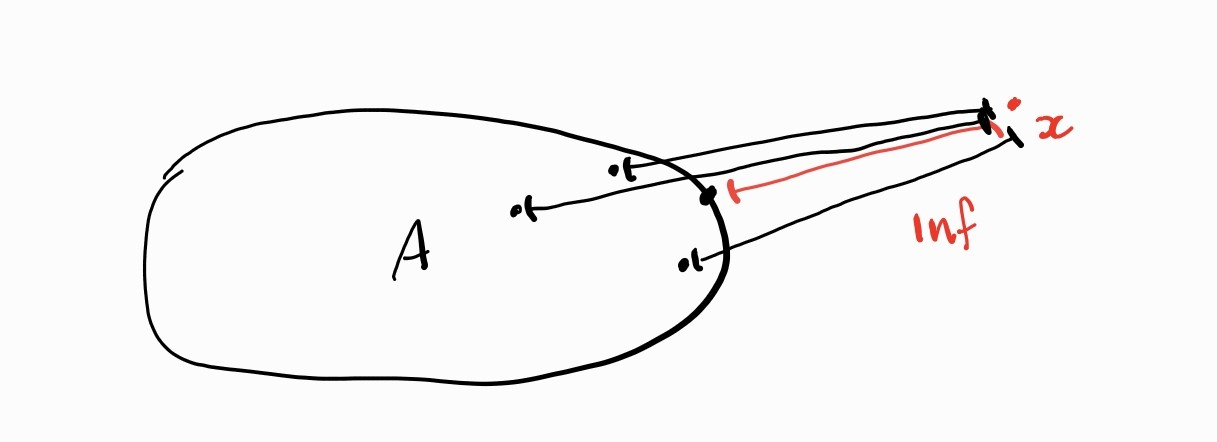
\includegraphics[width=0.5\linewidth]{images/dist-point.jpg}
    \label{fig:placeholder}
\end{figure}

\[ d(A,x) = \inf\{d(x,y) : y \in A\} \]
and continue with the distance between two subsets $A,B \subseteq X$:

\begin{figure}[h]
    \centering
    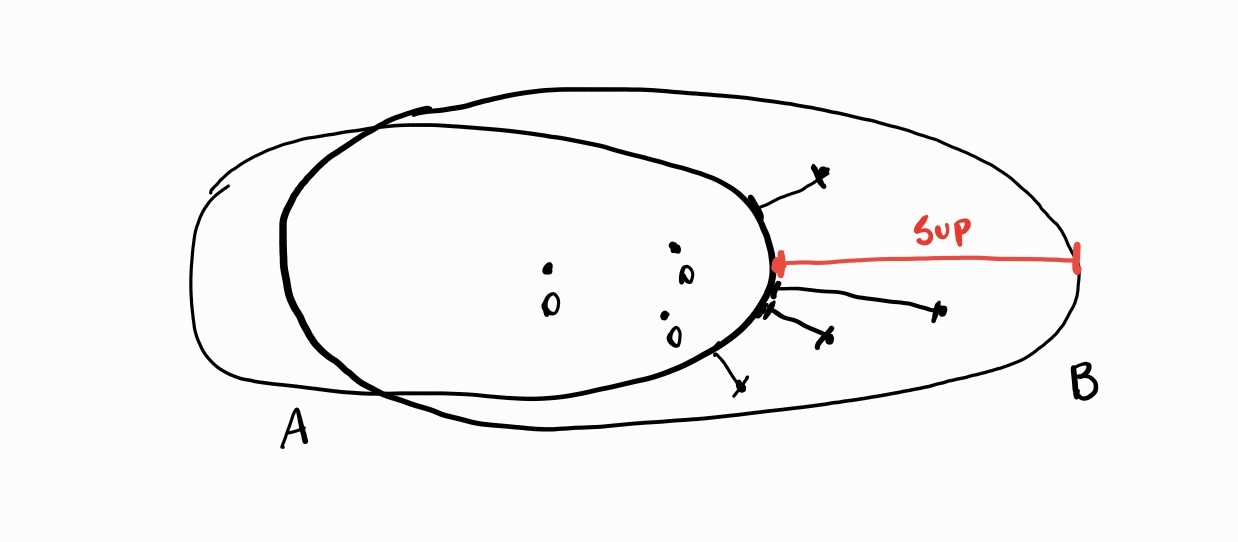
\includegraphics[width=0.5\linewidth]{images/dist-sets2.jpg}
    \label{fig:placeholder}
\end{figure}
\newpage
\[ d(A,B) = \sup\{d(A,x) : x \in B\} \]


Now, in order to ensure symmetry, we need to compare the distances $d(A,B)$ and $d(B,A)$, resulting exactly in the definition we wanted for the first image
\[ H(d)(A,B) = \max\{d(A,B),d(B,A)\} \]
$H(d)$ is known as the \textbf{Hausdorff lifting of $d$}.
Finally, one can prove that, starting with a 1-bounded metric space $(X,d)$, we have that $(\mathcal{P}(X),H(d))$ is also a 1-bounded metric space.

Now, for the functor $\mathcal{D}$ we need a more elaborated example in order to understand the intuition behind the lifting (we follow \cite[Section 2.1]{coalg-metrics}).  

Suppose you are the owner of three coffee roasting plants, $A,B$ and $C$, each with an adjacent café where one can taste the coffee. We let $X = \{A,B,C\}$ be the set of places and consider the distributions $P \colon X \to [0,1]$ and $Q \colon X \to [0,1]$ below to model supply and demand, respectively, of each product in proportion to the total supply or demand:

\[\begin{array}{cccccccccc}
    & P \colon & X & \longrightarrow         &  [0,1] & & Q \colon & X & \longrightarrow         &  [0,1]\\
    \\
    &         & A             & \longmapsto &  0.7 &     &    & A             & \longmapsto &  0.2 \\
    \\
    &         & B              & \longmapsto &  0.1 & &         & B              & \longmapsto &  0.3\\
    \\
    &         & C              & \longmapsto &  0.2 & &         & C              & \longmapsto &  0.5\\
    \end{array}\]
(For the sake of simplicity,
we assume that the total amount of production equals the amount of consumption.)

We have illustrated this situation graphically below. The numbers on the edges indicate the distance between the places $A$, $B$ and $C$ (the distance between a place and itself is $0$) whereas the numbers on the nodes indicate supply $P$ (upper value) and
demand $Q$ (lower value):

\begin{center}
        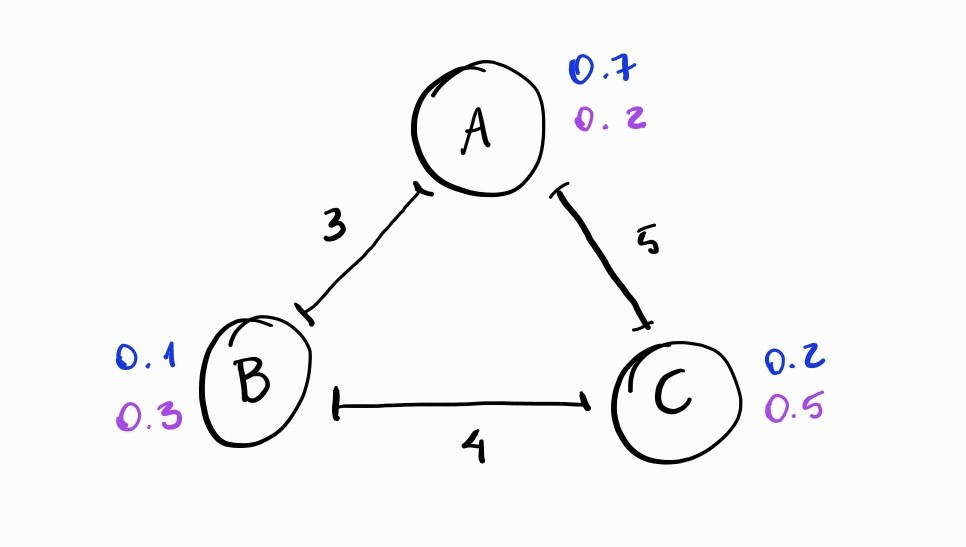
\includegraphics[width=0.5\linewidth]{images/kant-lift.jpg}
\end{center}
   

The goal is to find a economically motivated view of defining a distance between $P$ and $Q$ based on the notion of transportation which is studied extensively in transportation theory \cite{Villani_2009}. The leading idea is that the product needs to be transported so as to avoid excess supply and meet all demands.

Formally, we will have to define a function $t \colon X \times X \to [0, 1]$ where $t(x, y)$ describes (in \%) the amount of goods to be transported from place $x$ to $y$ such that:
\begin{itemize}
    \item supplies are used up: for all $x \in X$ we must have $\sum_{y \in X} t(x, y) = P (x)$;
    \item demand is satisfied: for all $y \in X$ we must have $\sum_{x\in X} t(x, y) = Q(y)$.
\end{itemize}

In probability theory, such a function is a joint probability distribution on $X \times X$ with marginals $P$ and $Q$ and is called a coupling of $P$ and $Q$. Here, we will call it a transportation plan for supply $P$ and demand $Q$ and write $T (P, Q)$ for the set of all such transportation plans.

Supposing the cost of transporting coffee from a place to another is directly proportional to the distance between the places, to minimize the costs we want to minimize $\sum_{x,y \in X} t(x,y) \cdot d(x,y)$ among all possible transportation plans. Having that in mind we define
\[ K(d)(P,Q) = \inf\{\sum_{x,y \in X} t(x,y) \cdot d(x,y) : t \in T (P, Q)\} \]

For a generic metric space $(X,d)$ and distributions $\varphi_1, \varphi_2 \in \mathcal{D}(X)$, we define
\[K(d)(\varphi_1,\varphi_2) = \inf_{t \in Coup(\varphi_1,\varphi_2)} (\sum_{(x_1,x_2) \in X \times X} t(x_1,x_2) \cdot d(x_1,x_2) )\]
where $Coup(\varphi_1, \varphi_2)$ is defined as the collection of couplings of $\varphi_1$ and $\varphi_2$, i.e., 
$$Coup(\varphi_1, \varphi_2) = \{t \in \mathcal{D}(X \times X) : \mathcal{D}(\pi_1)(t) = \varphi_1 \text{ and } \mathcal{D}(\pi_2)(t) = \varphi_2\}$$ where $\pi_1 : X_1 \times X_2 \to X_1$ and $\pi_2 : X_1 \times X_2 \to X_2$ are the projection functions. These are the generic equivalent of using all the supplies and satisfying all demands as exemplified above.
$K(d)$ is known as the \textbf{Kantorovich lifting of $d$}.
Starting with a 1-bounded metric space $(X,d)$, one can prove that $(\mathcal{D}(X),K(d))$ is also a 1-bounded metric space.

Since $\C(X) \subseteq \mathcal{P}\mathcal{D}(X)$ we can use these two liftings to define a distance function for $\C(X)$, that is we can show that $(C(X), HK(d))$ is a 1-bounded metric space. This gives us our desired $\cat{1Met}$-monad $\hat \C$, which has the same action on arrows and same unit and multiplication as the monad $\C$.

\paragraph{What about presentations?}

Now, the difference in considering program distances instead of program equivalence is expressed also algebraically. Instead of describing the axioms using equality ``$=$'', we use relations $a =_{\varepsilon} b$ which we think of as saying that ``$a$ is equal to $b$ up to an error of $\varepsilon$".  

We replace equalities by quantitative inferences:
$$\{x_i =_{\varepsilon_i} y_i\}_{i\in I} \vdash s =_{\varepsilon} t$$ where $\varepsilon$, $\varepsilon_i \in [0,1]$ and $s, t$ are terms. 



A quantitative inference is satisfied in a quantitative algebra $(A, {f^A}_{f \in \Sigma},d)$, where the maps $f^A$ are non-expansive and $(A,d) \in \cat{1Met}$, if, for all $x_i,y_i,s,t \in A$, we have:

\[ \text{if } d(x_i, y_i) \leq \varepsilon_i \text{ for all } i \in I, \text{ then } (s, t) \leq \varepsilon.\]

Similarly, we replace algebraic theories by quantitative equational theories.
 For instance, the quantitative equational theory of convex semilattices has signature $\Sigma_CS = (\{\oplus\}\cup\{+_p\}_{p\in(0,1)})$ and is defined as the set of quantitative inferences derivable by the following axioms, stated for arbitrary $p, q \in (0, 1)$ and $\varepsilon_1, \varepsilon_2 \in [0, 1]$:
    we substitute every axiom $A,C,I,A_p,C_p,I_p$ and $D$ in \(\Th_{CS}\) by changing the usual equality ``$=$'' for the inference $ \emptyset \vdash $ with $=_0$
    \[\begin{aligned}
&\text{(A)} && \emptyset \vdash x \oplus (y \oplus z) =_{0} (x \oplus y) \oplus z \\
&\text{(C)} && \emptyset \vdash x \oplus y = y \oplus x \\
&\text{(I)} && \emptyset \vdash x \oplus x = x \\
&\text{(A}_p) && \emptyset \vdash (x +_q y) +_p z = x +_{pq} (y +_{\frac{1-q}{1-p}} z) \\
&\text{(C}_p) && \emptyset \vdash x +_p y = y +_{1-p} x \\
&\text{(I}_p) && \emptyset \vdash x +_p x = x \\
&\text{(D)} && \emptyset \vdash x +_p (y \oplus z) = (x +_p y) \oplus (x +_p z) \\
\end{aligned}\]
    and add the following quantitative inferences
    \[\begin{aligned}
&\text{(H)} && \{x_1 =_{\varepsilon_1} y_1, x_2 =_{\varepsilon_2} y_2\} \vdash x_1 \oplus x_2 =_{max(\varepsilon_1,\varepsilon_2)} y_1 \oplus y_2 \\
&\text{(K)} && \{x_1 =_{\varepsilon_1} y_1, x_2 =_{\varepsilon_2} y_2\} \vdash x_1 +_p x_2 =_{p \cdot \varepsilon_1 + (1-p) \cdot \varepsilon_2} y_1 +_p y_2 
\end{aligned}\]

A model of a quantitative equational theories is then a quantitative algebra: a $\cat{1Met}$ space $A$ with a non-expensive function for all symbols of the theory, such that for every inference $\{x_i =_{\varepsilon_i} y_i\}_{i\in I} \vdash s =_{\varepsilon} t$, and variables $x_i, y_i$ in $A$, if $d(x_i, y_i) \leq \varepsilon_i$ for all $i \in I$, then $d(s,t)\leq \varepsilon$ when we interpret the variables $x_i$ and $y_i$ by the corresponding points in $A$, and the symbols by the corresponding functions on $A$.

\paragraph{Lifting termination.}


As in the $\cat{Set}$ case, there is also a termination monad $+\hat 1$ that can be composed with any $\cat{1Met}$ monad. We thus get a monad $\hat \C(+ \hat 1)$ for free.

% As in the $\cat{Set}$ case, the termination monad $+\hat 1$ on $\cat{1Met}$ also admits a monad distributive law with any  $\cat{1Met}$-monad, and we thus get a monad $\hat \C(+ \hat 1)$ for free. We denote $in_l \colon X \to X + \hat 1$ and $in_r \colon \hat 1 \to X + \hat 1$ the left and right coproduct injections, respectively. Then we can use the distributive law
% \[ \lambda \colon [\hat{\C} (in_l), \eta^{\hat{\C}}_{X+\hat{1}} \circ in_r] \]
% given by the diagram
% \[% https://tikzcd.yichuanshen.de/#N4Igdg9gJgpgziAXAbVABwnAlgFyxMJZARgBoAGAXVJADcBDAGwFcYkQAdDgC3p2C4BhAL4AKABoBqLr37FhAShDDS6TLnyEU5UsWp0mrdjL4COIiUpVrseAkTJ6aDFm0ScepoWPELpnuWFlVRAMW00iACZdfRcjdxNA5X0YKABzeCJQADMAJwgAWyQyEBwIJB0DV2MAswssMAB9RisQvMKkaNLyxErGBrcQKHo4blSQGkZ6ACMYRgAFdTstEFysNO4cCar4jymC6eHgnPyixABmGjKKyZm5xfD7dzWNredDQa4YHHoAPTNZHVhI1gFJEsB5MJhAACLgAYywuTh0IajVyxxA7TOJWuiEi1kxpyQl26nWElGEQA
% \begin{tikzcd}
%                                                    & \hat{\C}(X+\hat{1})                               &                                                                         \\
% \hat{\C}(X) \arrow[ru, "\hat{\C}(in_l)"] \arrow[r] & \hat{\C}(X)+\hat{1} \arrow[u, "\lambda"', dashed] & \hat{1} \arrow[lu, "\eta^{\hat{\C}_{X+\hat{1}}} \circ in_r"'] \arrow[l]
% \end{tikzcd}\]
% We have that $\hat{\C}(+\hat{1})$ is a monad with 
% $$\eta^{\hat{\C}(+\hat{1})} = \eta^{\hat{\C}} * \eta^{\hat{1}} ~\text{ and }~\mu^{\hat{\C}(+\hat{1})} = \mu^{\hat{\C}}*\mu^{\hat{1}} \circ \hat{\C} \lambda (+\hat{1})$$
% where $*$ is the horizontal composition of natural transformations, resulting in
% \[\eta^{\hat{\C}(+\hat{1})} \colon X \xrightarrow{\eta^{\hat{\C}_X}} \hat{\C}(X) \xrightarrow{\hat{\C}(\eta^{+\hat{1}})} \hat{\C}(X + \hat{1})\]
% and $\mu^{\hat{\C}(+\hat{1})}$ given by
% \[ \hat{\C}(\hat{\C}(X+\hat{1}) + \hat{1}) \xrightarrow{\hat{\C}(\lambda_{X+\hat{1}})} \hat{\C}(\hat{\C}((X + \hat{1})+\hat{1})) \xrightarrow{\mu^{\hat{\C}}_{(X+\hat{1})+\hat{1}}} \hat{\C}((X + \hat{1})+\hat{1}) \xrightarrow{\hat{\C}(\mu^{+\hat{1}}_{X})} \hat{\C}(X+\hat{1})\]

$\hat{\C}(+\hat{1})$ is also nicely presented by the quantitative equational theory of \emph{pointwise} convex semilattices, mirroring the $\cat{Set}$-case! For the $\mathcal C^\downarrow$ monad, more work is needed to provide a semantic description of the $\cat{1Met}$-monad $\hat{\mathcal C^\downarrow}$ presented by quantitative equational theory of pointed convex semilattices with the additional quantitative inference 
\[\begin{aligned}
&(\bot_\text{Q}) && \emptyset \vdash x \oplus \star =_0 x. 
\end{aligned}\]
As for the $\mathcal C+1$ monad, however, if we also add the quantitative inference
\[\begin{aligned}
&(\text{BH}_\text{Q}) && \emptyset \vdash x+_p \star =_0 \star 
\end{aligned}\]
for $p \in (0,1)$, then the result theory collapses: the quantitative $\emptyset \vdash x =_0 y$ is derivable, i.e. the underlying metric space is a point!

%\todo{For later, might be intersting to consider whether adding back A and O works in 1Met}

\bibliography{biblio}
\bibliographystyle{acm}

\end{document}
